% GNUPLOT: LaTeX picture with Postscript
\begingroup
  \makeatletter
  \providecommand\color[2][]{%
    \GenericError{(gnuplot) \space\space\space\@spaces}{%
      Package color not loaded in conjunction with
      terminal option `colourtext'%
    }{See the gnuplot documentation for explanation.%
    }{Either use 'blacktext' in gnuplot or load the package
      color.sty in LaTeX.}%
    \renewcommand\color[2][]{}%
  }%
  \providecommand\includegraphics[2][]{%
    \GenericError{(gnuplot) \space\space\space\@spaces}{%
      Package graphicx or graphics not loaded%
    }{See the gnuplot documentation for explanation.%
    }{The gnuplot epslatex terminal needs graphicx.sty or graphics.sty.}%
    \renewcommand\includegraphics[2][]{}%
  }%
  \providecommand\rotatebox[2]{#2}%
  \@ifundefined{ifGPcolor}{%
    \newif\ifGPcolor
    \GPcolorfalse
  }{}%
  \@ifundefined{ifGPblacktext}{%
    \newif\ifGPblacktext
    \GPblacktexttrue
  }{}%
  % define a \g@addto@macro without @ in the name:
  \let\gplgaddtomacro\g@addto@macro
  % define empty templates for all commands taking text:
  \gdef\gplbacktext{}%
  \gdef\gplfronttext{}%
  \makeatother
  \ifGPblacktext
    % no textcolor at all
    \def\colorrgb#1{}%
    \def\colorgray#1{}%
  \else
    % gray or color?
    \ifGPcolor
      \def\colorrgb#1{\color[rgb]{#1}}%
      \def\colorgray#1{\color[gray]{#1}}%
      \expandafter\def\csname LTw\endcsname{\color{white}}%
      \expandafter\def\csname LTb\endcsname{\color{black}}%
      \expandafter\def\csname LTa\endcsname{\color{black}}%
      \expandafter\def\csname LT0\endcsname{\color[rgb]{1,0,0}}%
      \expandafter\def\csname LT1\endcsname{\color[rgb]{0,1,0}}%
      \expandafter\def\csname LT2\endcsname{\color[rgb]{0,0,1}}%
      \expandafter\def\csname LT3\endcsname{\color[rgb]{1,0,1}}%
      \expandafter\def\csname LT4\endcsname{\color[rgb]{0,1,1}}%
      \expandafter\def\csname LT5\endcsname{\color[rgb]{1,1,0}}%
      \expandafter\def\csname LT6\endcsname{\color[rgb]{0,0,0}}%
      \expandafter\def\csname LT7\endcsname{\color[rgb]{1,0.3,0}}%
      \expandafter\def\csname LT8\endcsname{\color[rgb]{0.5,0.5,0.5}}%
    \else
      % gray
      \def\colorrgb#1{\color{black}}%
      \def\colorgray#1{\color[gray]{#1}}%
      \expandafter\def\csname LTw\endcsname{\color{white}}%
      \expandafter\def\csname LTb\endcsname{\color{black}}%
      \expandafter\def\csname LTa\endcsname{\color{black}}%
      \expandafter\def\csname LT0\endcsname{\color{black}}%
      \expandafter\def\csname LT1\endcsname{\color{black}}%
      \expandafter\def\csname LT2\endcsname{\color{black}}%
      \expandafter\def\csname LT3\endcsname{\color{black}}%
      \expandafter\def\csname LT4\endcsname{\color{black}}%
      \expandafter\def\csname LT5\endcsname{\color{black}}%
      \expandafter\def\csname LT6\endcsname{\color{black}}%
      \expandafter\def\csname LT7\endcsname{\color{black}}%
      \expandafter\def\csname LT8\endcsname{\color{black}}%
    \fi
  \fi
    \setlength{\unitlength}{0.0500bp}%
    \ifx\gptboxheight\undefined%
      \newlength{\gptboxheight}%
      \newlength{\gptboxwidth}%
      \newsavebox{\gptboxtext}%
    \fi%
    \setlength{\fboxrule}{0.5pt}%
    \setlength{\fboxsep}{1pt}%
    \definecolor{tbcol}{rgb}{1,1,1}%
\begin{picture}(6802.00,5102.00)%
    \gplgaddtomacro\gplbacktext{%
      \csname LTb\endcsname%%
      \put(1036,1456){\makebox(0,0)[r]{\strut{}$0,6$}}%
      \csname LTb\endcsname%%
      \put(1036,2129){\makebox(0,0)[r]{\strut{}$0,7$}}%
      \csname LTb\endcsname%%
      \put(1036,2802){\makebox(0,0)[r]{\strut{}$0,8$}}%
      \csname LTb\endcsname%%
      \put(1036,3475){\makebox(0,0)[r]{\strut{}$0,9$}}%
      \csname LTb\endcsname%%
      \put(1036,4148){\makebox(0,0)[r]{\strut{}$1$}}%
      \csname LTb\endcsname%%
      \put(1036,4821){\makebox(0,0)[r]{\strut{}$1,1$}}%
      \csname LTb\endcsname%%
      \put(1204,1176){\makebox(0,0){\strut{}$0,4$}}%
      \csname LTb\endcsname%%
      \put(1841,1176){\makebox(0,0){\strut{}$0,5$}}%
      \csname LTb\endcsname%%
      \put(2477,1176){\makebox(0,0){\strut{}$0,6$}}%
      \csname LTb\endcsname%%
      \put(3114,1176){\makebox(0,0){\strut{}$0,7$}}%
      \csname LTb\endcsname%%
      \put(3750,1176){\makebox(0,0){\strut{}$0,8$}}%
      \csname LTb\endcsname%%
      \put(4387,1176){\makebox(0,0){\strut{}$0,9$}}%
      \csname LTb\endcsname%%
      \put(5024,1176){\makebox(0,0){\strut{}$1$}}%
      \csname LTb\endcsname%%
      \put(5660,1176){\makebox(0,0){\strut{}$1,1$}}%
      \csname LTb\endcsname%%
      \put(6297,1176){\makebox(0,0){\strut{}$1,2$}}%
    }%
    \gplgaddtomacro\gplfronttext{%
      \csname LTb\endcsname%%
      \put(266,3138){\rotatebox{-270}{\makebox(0,0){\strut{}$\bar{\pi}_\text{ст}$}}}%
      \put(3750,756){\makebox(0,0){\strut{}$\bar{G}$}}%
      \csname LTb\endcsname%%
      \put(5226,483){\makebox(0,0)[r]{\strut{}гладкие лопатки}}%
      \csname LTb\endcsname%%
      \put(5226,203){\makebox(0,0)[r]{\strut{}турбулизаторы}}%
      \put(70mm,44mm){\makebox(0,0)[l]{\strut{}$\bar{n} = 0.69$}}%
      \put(78mm,63mm){\makebox(0,0)[l]{\strut{}$\bar{n} = 0,82$}}%
      \put(88mm,78mm){\makebox(0,0)[l]{\strut{}$\bar{n} = 1,00$}}%
    }%
    \gplbacktext
    \put(0,0){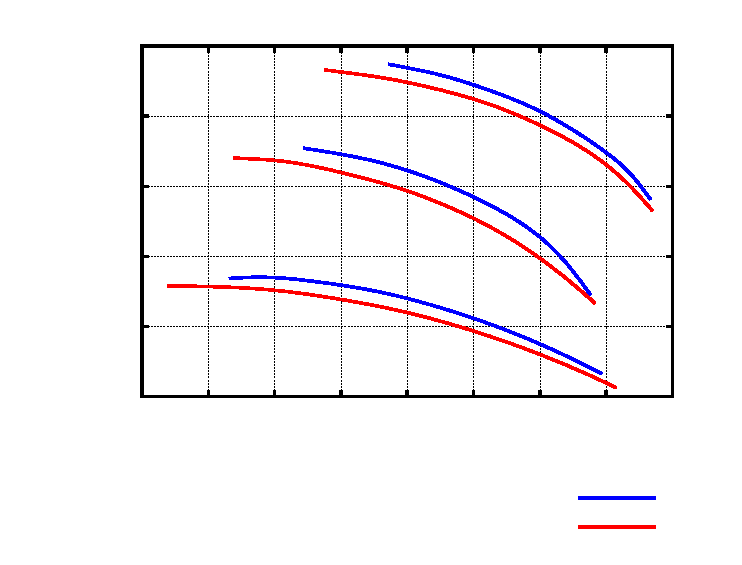
\includegraphics[width={340.10bp},height={255.10bp}]{teresch1988turb}}%
    \gplfronttext
  \end{picture}%
\endgroup
